\documentclass[12pt]{report}
\usepackage[a4paper, width=150mm, top=25mm, bottom=25mm, headheight=20mm]{geometry}
\usepackage[backend=biber, style=numeric, sorting=none]{biblatex}
\usepackage{graphicx}
\usepackage{fancyhdr}
\usepackage{amsmath}
\usepackage{parskip}
\usepackage[table,xcdraw]{xcolor}
\usepackage{longtable}
\usepackage{soul}  % For highlighting text - remove when done
\usepackage{hyperref}
\usepackage[explicit,compact]{titlesec}
\usepackage{pdfpages}
\usepackage{multicol}
\usepackage{csquotes}

\hypersetup{colorlinks=true, linkcolor=black, citecolor=black, urlcolor=blue}
\graphicspath{{./images/}}
\counterwithout{figure}{chapter}
\counterwithout{table}{chapter}
\addbibresource{citations.bib}
\titleformat{\chapter}[block]{\bfseries\huge}{\filright\huge\thechapter.}{1ex}{\huge\filright #1}
\titlespacing*{\chapter}{0pt}{4ex plus 1ex minus .2ex}{3.8ex plus .2ex}
\titlespacing*{\section}{0pt}{3.5ex plus 1ex minus .2ex}{1.8ex plus .2ex}
\titlespacing*{\subsection}{0pt}{3.0ex plus 1ex minus .2ex}{1.3ex plus .2ex}

\renewcommand{\chaptermark}[1]{\markboth{#1}{}}

% For highlighting text - remove when done
\newcommand{\hlc}[2][yellow]{{%
    \colorlet{foo}{#1}%
    \sethlcolor{foo}\hl{#2}}%
}

\pagestyle{fancy}
\fancyhead[L]{From Scramble to Solution}
\fancyhead[R]{\leftmark}
\fancyfoot[C]{\thepage}

\title{From Scramble to Solution: Developing an Optimal Solver for the Kilominx, a Rubik's Cube Variant}
\author{Samuel Borg}
\date{\today}

\begin{document}

\begin{titlepage}
    \begin{center}
        \vspace*{1.5cm}
            
        \Huge
        \textbf{From Scramble to Solution}
            
        \vspace{0.5cm}
        \LARGE
        Developing an Optimal Solver for \\ the Kilominx, a Rubik's Cube Variant

        \vspace{2cm}
        \textbf{Samuel Borg}

        \Large
        \textit{Supervisor: Ian Gent}

        \vspace{0.5cm}

        \large
        \today

        \vspace{2.5cm}

        
\includegraphics[width=0.4\textwidth]{unilogo}

        \Large
        \vspace{0.5cm}
        School of Computer Science\\
        University of St Andrews
    \end{center}
\end{titlepage}

\chapter*{Abstract}
The Rubik's Cube is the most well-known combination puzzle of all time, and has inspired numerous variants of the puzzle. One such puzzle is the Kilominx, a 2x2 dodecahedron-shaped puzzle with 12 faces and 20 cubies (individual cube elements of the puzzle). While the Rubik's Cube has already been extensively researched, the Kilominx has not.

This report details my work in creating an optimal solver for the Kilominx, guaranteeing solutions in as few moves as possible. A separate program I wrote precomputes several pattern databases, each containing the number of moves required to solve different subsets of cubies in all possible states. The solver uses an iterative-deepening A* (IDA*) algorithm to find the optimal solution, using the pattern databases as a lower-bound heuristic. In order to efficiently index into the pattern databases, the solver computes a Lehmer code for the puzzle state, which is then used to calculate the state's sequential index.

In theory, the solver could optimally solve any state given enough time, but in practice it can only find solutions up to a depth of 14 within a reasonable timeframe. As solutions require longer sequences of moves to solve, the solver takes exponentially more time to find the optimal solution. Results from the solver demonstrate that it is unlikely an optimal solver could be used to help tighten the bounds on the Kilominx's God's Number - the maximum number of moves needed to solve the puzzle from any given state.

\chapter*{Declaration}
I declare that the material submitted for assessment is my own work except where credit is explicitly given to others by citation or acknowledgement. This work was performed during the current academic year except where otherwise stated.

The main text of this project report is 10,635 words long, including project specification and plan.

In submitting this project report to the University of St Andrews, I give permission for it to be made available for use in accordance with the regulations of the University Library. I also give permission for the title and abstract to be published and for copies of the report to be made and supplied at cost to any bona fide library or research worker, and to be made available on the World Wide Web. I retain the copyright in this work.

\chapter*{Acknowledgements}
I would like to thank my supervisor, Ian Gent, for his invaluable guidance, insight and support throughout this project. His expertise and enthusiasm have made this project an incredibly engaging and rewarding journey.

I would also like to thank my parents, Juliet and Peter, my brother, Tom, and my amazing friends Emil, Ben, Zoe, Josh, Maya, Jess and Alfie for their unwavering support and belief in me all the way through my studies.

\tableofcontents

\chapter{Introduction}
% Describe the problem you set out to solve and the extent of
% your success in solving it. You should include the aims and
% objectives of the project in order of importance and try to
% outline key aspects of your project for the reader to look for
% in the rest of your report.

When the Rubik's Cube was globally released in 1980, it became an instant success, selling around 200 million units by the end of 1983 \cite{unitssold}. The Rubik's Cube also quickly became a popular subject of research for computer scientists, in part due to the massive 43 quintillion possible states \cite{states} that the cube can be in. Many different algorithms were designed to try and solve the cube in as few a number of moves as possible, but it wasn't until 1997 that Richard E. Korf published a paper \cite{korf} describing a method to solve the Rubik's Cube optimally (the shortest possible number of moves to solve any given cube state) by using large lookup tables called pattern databases\cite{patterndatabases} as a heuristic function to guide an IDA* search algorithm. 

% god number stuff here

The widespread success of the Rubik's Cube also led to the creation of a number of different variants of the puzzle, each working similarly to the Rubik's Cube but of different shapes and sizes. The Kilominx is one of these variants, part of the larger "minx" family of dodecahedron-shaped puzzles. The Kilominx is a 2x2 dodecahedral puzzle with 12 faces and 20 cubies (the individual cube-shaped elements of the puzzle). Although some research has been done on tightening the bounds of its God's Number, no optimal solver has previously been created for the puzzle.

\begin{figure}[h]
    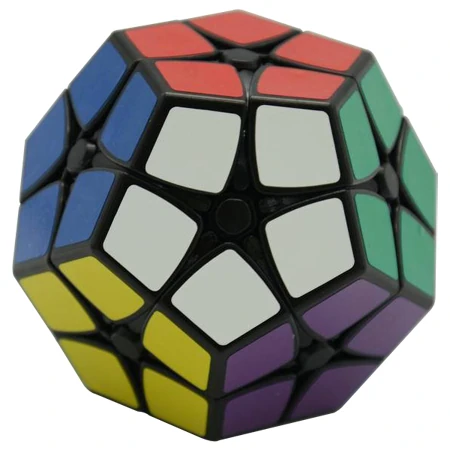
\includegraphics[width=0.4\textwidth]{kilominx}
    \centering
    \caption{An image of a Kilominx.}
    % Image URL: https://static.wikia.nocookie.net/speedcubesolving/images/8/88/4941_P_1467693201156-1-.jpg/revision/latest?cb=20180218173628
    % Website URL: https://speedcubesolving.fandom.com/wiki/Kilominx
\end{figure}

\section{Objectives}

\chapter{Context Survey}
% Surveying the context, the background literature and any
% recent work with similar aims. The context survey describes
% the work already done in this area, either as described in
% textbooks, research papers, or in publicly available software.
% You may also describe potentially useful tools and
% technologies here but do not go into project-specific
% decisions.

\section{Korf's Algorithm for the Rubik's Cube}
% Go into detail about Korf's paper for the rubik's cube. Mention any important design decisions he made. Relate it to what I am doing.
\subsection{Iterative-Deepening A*}
\subsection{Pattern Databases}
% Small section here about the other pattern databases paper. Why use pattern databases?

\subsection{Sequential Indexing with Lehmer Codes}
% Again, more here to do with sequential indexing and lehmer codes. Use Korf's other paper, and possibly the article that explains it.

\section{God's Number}
% What research has been done on God's Number for the cube and the kilominx? What methods were used? How does it relate to what I'm doing?

\section{The Kilominx}
% Any research on the Kilominx?

\chapter{Requirements Specification}
% Capturing the properties the software solution must have in
% the form of requirements specification. You may wish to
% specify different types of requirements and given them
% priorities if applicable.

\chapter{Software Engineering Process}
\section{Software Development Process}
An incremental development process was used for this project in order to ensure steady progress throughout both semesters. This approach allowed me to slowly build up the solver in small, functional increments, where each increment was thoroughly tested and documented before moving on to the next. This method helped ensure that the final solution was robust and well-documented.

At the start of the project, I began by creating a reference guide for creating an optimal solver for the Rubik's Cube. This guide detailed each of the steps required to model the Rubik's Cube and then create the optimal solver for it, highlighting any important design decisions that needed to be made along with concise justifications for the decisions. This guide was used as a roadmap for the development of the solver, ensuring that I stayed on track towards the final goal.

After creating the reference guide, I followed it to implement an optimal solver for the Rubik's Cube. While creating a solver for the Rubik's Cube was not part of the project objectives, it was a necessary step in order to gain a better understanding of the process required to create an optimal solver. I took care while implementing the classes and methods to ensure that they were modular and reusable - this allowed me to easily extend the both the solver and other classes to work with the Kilominx later on. The Rubik's Cube solver was thoroughly tested to ensure that it was working correctly before moving on to implementing the Kilominx solver.

Finally, I implemented the Kilominx solver following the same steps from the reference guide as I did for the Rubik's Cube solver. I reused many of the classes and methods from the Rubik's Cube solver, extending them where necessary to work with the Kilominx. The Kilominx solver was also thoroughly tested to ensure that it was working correctly.

\section{Choice of Language}
I decided to use Java as the primary programming language for the solver. This decision was made based on my familiarity with Java and its object-oriented principles, such as abstract classes and inheritance, which I believed would be helpful for allowing parts of the code to be reused and extended. Additionally, Java is a relatively fast language and is well-suited for the type of computation required for solving the Rubik's Cube and Kilominx. There was some consideration given to using C++ due to its speed and efficiency, but due to my lack of experience with the language, I ultimately decided that Java would be the best choice for this project.


\chapter{Ethics}
The original project objectives involved surveying users about their experience with the web application, so the Artefact Evaluation form was filled out and submitted. However, as this objective was moved down to a lower priority, the user survey was ultimately not conducted. The Artefact Evaluation form can be found in \textbf{\hyperref[appendix:artefact]{Appendix A}}.

\chapter{Design \& Implementation}
\section{Modelling the Puzzles}
In order to ensure both the Rubik's Cube and the Kilominx can be used interchangeably in the code for populating pattern databases and with the IDA* search algorithm, an interface is defined to represent a "twisty puzzle", which both the Rubik's Cube and Kilominx implement. Similar interfaces are defined for the move controllers, moves and colours in order to ensure that the code is as reusable as possible. 

\subsection{Representing the State for a Rubik's Cube}
The state of the Rubik's Cube was modelled similarly to how it was described by Korf in his paper \cite{korf}, but with some changes. Instead of using a single array for all 20 cubies, I chose to use two arrays: one for the 12 edge cubies and the other for the 8 corner cubies. This improves the clarity of the code without a significant compromise on speed/efficiency. Representing the cube as arrays of cubies allows for very quick manipulation of the cube. This is important later on for the IDA* algorithm, as moves need to be made on the cube many, many times - the faster the moves can be performed, the faster the IDA* algorithm will be able to search for an optimal solution.

% ADD A DIAGRAM OF A RUBIK'S CUBE WITH CUBIE LABELS

Cubies are modelled as a class with two fields: an index (which signifies the cubie's initial position and colours) and an orientation. Since the maximum value for the index is 19 and the maximum value for the orientation is 2, both fields can fit comfortably in byte data types. This reduces how much memory is required to store a cube state.

For each corner and edge cubie on the cube, there is an associated constant value which holds the cubie's initial position in the corner/edge array. These constants are used when accessing cubies at specific positions in order to increase readability (e.g. instead of accessing the cubie at index 0, access the cubie at position CORNER\_ULB).

The initial state (or the solved state) of the cube is defined with the white face on top and the red face at the front. Since the centre cubies of the faces can not move, each physical cube state can only be represented by the code in a single way. Therefore, the only way to represent a solved cube state is with the white face on top and the red face at the front. This makes it easier to check if a cube is solved, and it also makes it easier to determine how many moves away a state is from being solved when creating the pattern databases.

The chosen values for the corner cubie indices are important, as they are used to correctly determine which colours should appear on which faces. Corner cubies which are an odd number of quarter turns away from each other should also be an odd number of indices apart in the array - the same applies for cubies which are an even number of quarter turns away being an even number of indices apart. For example, the cubie in the up-left-back (ULB) corner can turn to the up-right-back (URB), up-left-front (ULF), and down-left-back (DLB) corners in a single quarter turn, and to the down-right-front (DRF) corner in three quarter turns; since the ULB cubie has an index of 0 (which is even), then the URB, ULF, DLB and DRF cubies should all be an odd number of indices away from 0.

When the cube is in a solved state, the initial orientation of all of the cubies is 0. Edge cubies can have an orientation of 0 (oriented) or 1 (flipped), where an edge is oriented if it can be solved using only U, D, L and R moves. Corner cubies can have an orientation of 0 (when the white/yellow side of the corner is on the top or bottom face), 1 (when the white/yellow side of the corner is on the face clockwise from the top or bottom face), or 2 (when the white/yellow side of the corner is on the face counter-clockwise from the top or bottom face).

An enum is defined which holds the six different colours on the cube - white (W), green (G), red (R), blue (B), orange (O) and yellow (Y). The subset of colours that appear on a cubie are determined by its index, and colours are always returned by helper functions in the following order: the colour on the top/bottom face first, then the colour on the front/back face, and finally the colour on the left/right face. The default order of colours for cubies in their initial positions with an orientation of 0 is pre-defined, making it easy to return the colours in the correct order. However, after cubies have been moved about and are in different positions/orientations, it becomes a little more complicated to determine which colours appear on which faces. For edge cubies, if the orientation of the edge is 1 (denoting a flipped orientation) then the colours are returned in reverse order. For corner cubies, the order is determined by the orientation of the corner, whether the cubie's current position has an even or odd index, and whether the cubie is an even or odd number of indices away from its initial position. The colours can then be used to print the cube's state in a human-readable format.

\subsection{Representing the State for a Kilominx}
The Kilominx is represented very similarly to the Rubik's Cube, but with some key changes. Since the Kilominx is made up of only "corner" cubies, I chose to represent the state as a single array of 20 cubies.

The initial state of the Kilominx is also defined with the white face on top and the red face at the front. However, since there are no centre cubies on a Kilominx, there is no easy way to figure out the correct orientation of a scrambled Kilominx. This also creates further problems when creating pattern databases later on, as each physical Kilominx state can be represented by the code in $60\ (= 20 \text{ cubies} \cdot 3 \text{ orientations})$ different ways. So to get around this problem, I chose to fix one of the cubies in place, such that it is always in the same position and orientation - all of the other cubies are defined relative to this cubie. I arbitrarily chose to fix the up-front-left (UFL) cubie. Now, each physical state can only be represented in the code in a single way.

The indices of the cubies are important again for determining colour orders, but the reasoning behind which cubies are even and which are odd is different for the Kilominx. The faces of the Kilominx have the following priority order (going from highest to lowest): top/bottom, left/down-back-right, front/down-back-middle, right/down-back-left, down-left/back-right, and down-right/back-left. This priority order is used for a few things, including the return order of colours from helper functions for printing the Kilominx's state. When the Kilominx is in the initial state, any cubies which return their colours in a counter-clockwise order have an even index, and any cubies which return their colours in a clockwise order have an odd index.

%  maybe put the face/colour priorities in a table here?

The priority order defined above is also used to determine the orientation of the cubies \cite{kilominxorientation}. In the same way that the faces have a priority order, the colours also have a priority order (which is in the same order as the faces when the Kilominx is in the initial state): white/grey, light/dark-green, red/orange, light/dark-blue, beige/yellow, and pink/purple. Looking at a single cubie, the face which the highest-priority colour is on is compared to the highest-priority face the cubie is part of. There are three different cases - if the highest-priority colour is on:
\begin{itemize}
    \item the highest-priority face, the cubie has an orientation of 0.
    \item the face clockwise from the highest-priority face, the cubie has an orientation of 1.
    \item the face counter-clockwise from the highest-priority face, the cubie has an orientation of 2.
\end{itemize}

% example of above?

A different enum is defined for the colours on a Kilominx: white (Wh), dark-green (DG), red (Re), dark-blue (DB), yellow (Ye), purple (Pu), light-blue (LB), beige (Be), pink (Pi), light-green (LG), orange (Or), and grey (Gy). Two characters are used for the Kilominx's colours to prevent confusion between colours that start with the same letter (e.g. 'G' could refer to dark-green, light-green, or grey). The method to determine which colours and what order to display them is the same as with the Rubik's Cube, albeit with some slight logic changes to match the priority orders defined above.

\subsection{Making Moves}
\label{subsection:moves}
Both the Rubik's Cube and the Kilominx hold a reference to a separate move controller object which contains all of the logic used to make moves on the puzzle. This logic is kept separate from the code used to define the Rubik's Cube and Kilominx in order to make the code more readable.

Both move controllers contain an enum which defines the available moves for the puzzle associated with the move controller. Each move has an associated inverse move (which defines the move that undoes it, e.g. $U'$ is the inverse of $U$) and a base move (which defines the face the move acts on, e.g. $F$ is the base move of $F2$ and $F'$).

Moves on the puzzles are made by performing the following basic operations on different cubies or sets of cubies:
\begin{itemize}
    \item Rotation of cubies: A set of cubies are swapped with each other in the cubie array, resulting in the positions of the cubies being "rotated" in a cycle.
    \item Edge orientation flip: The orientation of an edge on the cube is flipped from 0 to 1, or from 1 to 0.
    \item Cubie orientation increase: The orientation of a corner on the cube or any cubie on the Kilominx is adjusted by adding either 1 or 2, and then is reduced by modulo 3 in order to keep the orientation within the range 0 to 2.
\end{itemize}
These three basic operations are enough to define any possible move on the puzzles. 

% example of a move?

For the Kilominx, moves which affect the fixed UFL cubie (any moves on the U, L and F faces) are performed as normal, but are then followed by a full rotation of the Kilominx in order to reposition the fixed cubie back to the UFL corner with the correct orientation. This allows the fixed cubie to move around the Kilominx relative to the rest of the cubies, while ensuring that each physical state can only be represented in one way.

As discussed by Korf in his paper \cite{korf}, when iterating over possible moves in the IDA* search, redundant moves can be skipped over in order to reduce the branching factor of the search. A move is skipped if the move is on the same face as the previous move, or if the move is on a non-adjacent face to the previous move and the moves are not performed in the correct order (up, left, front, right, back-left, back-right, down-left, down-right, down-back-left, down-back-right, down-back, down). For example, on a Kilominx, if the previous move was on the down-left (DL) face, and the next move is on the up (U) face, then the move will be skipped as the moves are not in the correct order. Java Streams are used to help simplify these checks, improving the clarity of the code.

\section{Pattern Databases}
Similar to how an interface is defined for a twisty puzzle, an abstract class is defined for a general pattern database. The abstract class contains implementation details which are the same for all pattern database subclasses, but cannot be directly instantiated because the way database indices are calculated differ slightly depending on the cubie selections for the pattern database subclasses.

A pattern database is essentially a large lookup table, which I chose to model as an array of bytes. Each table contains the number of moves required to solve a specific pattern - a subset of cubies (which are different depending on which pattern database subclass is used and what parameters are provided to the subclass constructor) - in every possible state, where each byte stores the number of moves for a single state. This results in a table that can be used as an admissible heuristic for the IDA* algorithm, as the number of moves required to solve any subset of cubies will always be less than or equal to the number of moves required to solve the entire puzzle state. Multiple pattern databases can be used together to improve the heuristic result by taking the maximum of the values returned by each pattern database for the current state.

Ideally we want the pattern databases to be as large as possible - the more cubies that are used in a pattern, the more accurate the heuristic becomes, which in turn improves the speed of the IDA* search. However, increasing the number of cubies used in a pattern exponentially increases the number of states (and so the amount of memory required to store the pattern database). So in practice, we should choose a number of cubies that is small enough to keep the pattern database in memory, but large enough to give a good heuristic.

We also need to decide what pattern of cubies we want to use for each pattern database. Culberson and Schaeffer note that "...experiments suggest that the best pattern databases are the ones that reduce the problem to a simpler one whose solution requires little or no interference with the placing of the target pattern." \cite{patterndatabases}. However, since every move for both the Rubik's Cube and the Kilominx affects the positions and orientations of cubies on multiple faces, there is no easy choice for a pattern of cubies to use. Korf chooses to make three pattern databases for the Rubik's Cube in his implementation: one containing all eight corner cubies, and two for the edge cubies (each containing six of the 12 edge cubies) \cite{korf}. This is a logical choice to make for the Rubik's Cube, as the corners and edges calculate their database indices slightly differently, but this isn't possible with the Kilominx as the puzzle is made up entirely of "corner" cubies, and as discussed above, we can't make a single pattern database for all of the Kilominx cubies as the table would require an absolutely enormous amount of memory.

For the Rubik's Cube, I chose to use three pattern databases in a similar manner to what Korf used: one with all eight corner cubies, and two with a number of edge cubies. However, since modern computers have far more memory than they did in 1995 (when Korf's paper was published), I was able to include seven edge cubies in each edge cubie pattern database (with two cubies appearing in both patterns). This gives a notable increase in speed for the IDA* search without requiring too much memory.

For the Kilominx, I chose to create two different pattern types for the pattern databases: the first selects five cubies that are part of the same face, and the second selects four cubies that are as far apart as possible. 12 face pattern databases are used - one for each face - and 5 sparse pattern databases are used - such that each cubie on the Kilominx appears in exactly one of these pattern databases. Using two different patterns and using a large number of them ensures many different states are covered, improving the accuracy of the heuristic. The number of cubies used in each pattern are also low enough to keep the size of the pattern databases small enough to fit in memory.

However, due to the fixed cubie in the UFL corner, some of the patterns used for the Kilominx pattern databases are slightly altered - this is because the fixed cubie is always in the same position and orientation, so it is no longer a part of the permutation of cubies for the pattern databases. Wherever the UFL cubie is used in a pattern database, it is instead replaced by a nearby cubie in order to keep the general pattern shapes consistent.

When a pattern database is initialised, we need to know how big the database will be ahead of time in order to create the array of bytes. This can be found by calculating the number of permutations that exist for the subset of cubies provided. For example, each Kilominx face pattern database considers 5 of the 19 cubies (excluding the 20th cubie, which is fixed in the UFL position), so the parameters $n$ and $k$ are set to 19 and 5 respectively. There are $^nP_k = {}^{19}P_5$ different permutations the cubies can be in (ignoring their orientations), and each of the 5 cubies can be in one of 3 orientations. Hence, the total number of states in the pattern database is $^{19}P_5 \cdot 3^5 = 339072480$.

\subsection{Database Index Calculation}
In order to calculate the database index for a given puzzle state, the Lehmer code of the permutation of the cubie indices used in the pattern is calculated and converted into base-10, and is then offset based on the permutation of the cubie orientations. This allows us to map each possible state for a pattern database to a unique index in the array.

The implementation follows the same linear algorithm outlined in \textbf{\hyperref[subsection:lehmercodes]{Section 2.1.4}}, but with some minor changes to improve its efficiency: the first digit of the Lehmer code isn't directly calculated because it is always equal to the first digit in the permutation, and instead of iterating through a bit string to count the number of ones that appear in it, we instead pre-compute a table which stores the number of ones that appear in the binary representations of all of the numbers that can be represented by the bit string, allowing for a constant lookup time. Similarly, a table is precomputed for all of the factorials that are needed to convert the Lehmer code into base-10 - by doing so ahead of time, we avoid needing to recursively calculate a factorial every time a database index is calculated.

\subsection{Populating Pattern Databases}
The pattern databases are populated using an iterative-deepening depth-first-search (IDDFS). While a breadth-first search (BFS) may initially seem like a better choice, the large branching factor of the puzzles (especially the Kilominx) mean that a very large number of states need to be kept in memory during search, which would eventually cause the BFS to run out of memory. Using an IDDFS means that only the path of states from the initial (solved) state to the current state needs to be kept in memory. However, this comes at the cost of search speed, as IDDFS will need to revisit lower depth states every time a depth level is completed.

Each node in the IDDFS search tree contains a puzzle state, the move used to get to the node, and the depth of the node. A stack is used to store the nodes, implemented using a double-ended queue (a deque). Starting with the node containing the initial puzzle state, nodes are popped off of the top of the stack and all possible moves from the node are iterated over (skipping moves where necessary, as explained in \textbf{\hyperref[subsection:moves]{Section 6.1.3}}), generating new nodes to push to the stack (up to the current depth limit). For each node that is encountered, the database value for the state is set to the number of moves needed to reach the state (the depth of the node). If the state had already been previously reached with a lower number of moves, then that value is kept instead. When the search tree has been fully explored up to the current depth limit, the depth limit is increased and the search repeats. This continues until every state has been reached and the pattern database is fully populated.

All of the pattern databases are populated ahead of time, as each IDDFS can take a long time to complete - especially for the larger Kilominx face pattern databases. Once all of the pattern databases have been populated, they do not need to be populated again.

\section{Searching for Solutions}
The puzzle solver is implemented as an abstract class, containing the bulk of the IDA* code, with the two subclasses containing code which is specific to the Rubik's Cube and Kilominx respectively (ensuring that they use the correct pattern databases).

The IDA* implementation is similar to the IDDFS implementation: nodes contain a puzzle state, the move used to get to the node, and the depth; the nodes are stored in a stack (implemented as a deque); nodes are generated by popping a node off of the top of the stack and iterating over all non-skipped moves; and the depth limit is increased whenever the current depth-bounded search tree is fully explored.

However, it differs from IDDFS in a few ways. First, the initial depth bound of the search is set to the maximum value returned by the pattern databases for the initial scrambled puzzle state. This helps reduce a lot of the unnecessary search at lower depth bounds, saving some time. Second, when new nodes are generated by iterating over moves from the current state, they are pushed to the stack in descending order of their estimated cost (implemented using a priority queue) - this results in the new top node of the stack having the lowest estimated cost, so the most promising area of the search tree is explored first. Third, newly generated nodes which have a greater estimated cost than the current bound get pruned from the search tree, ensuring that only nodes within the current bound limit are explored.

Once the solved state has been found, the IDA* search returns the solution path from the initial state to the solved state. The solution is guaranteed to be optimal, as the pattern databases are admissible heuristics.

\section{Interacting with the Puzzles}
A number of classes are defined to provide a way for the user to interact with the puzzles and the solvers.

The two terminal classes provide a command-line interface (CLI), allowing the user to view the current puzzle state in a human-readable format, make moves, and enter commands to manipulate the puzzles, including scrambling the puzzle with a specified number of moves, invoking the solver for the current puzzle state, and editing the current puzzle state. The edit command ensures that the new state is valid and can be solved by checking for duplicate cubies and performing the following parity checks \cite{parity}:
\begin{itemize}
    \item Corner Parity: the sum of the orientations of the corner cubies for the Rubik's Cube, or all cubies for the Kilominx, must be a multiple of 3.
    \item Edge Parity: the sum of the orientations of the edge cubies for the Rubik's Cube must be even.
    \item Permutation Parity: the sum of the number of swaps needed to place all of the cubies in their correct positions must be even.
\end{itemize}
In addition to this, the edit command doesn't allow the user to edit any fixed cubies, such as the centre cubies on the Rubik's Cube or the fixed cubie in the UFL corner on the Kilominx. This ensures that the orientation of the puzzle cannot be manually changed.

The GUI class provides a graphical user interface for the Rubik's Cube, providing mostly the same functionality as the CLI but with a better way of displaying the current cube state, and various hotkeys to allow the user to quickly make moves on the cube. The GUI was made with Java's Swing library, where the main window extends a JFrame and is composed of JPanels - one which contains the display of the cube state, and another which contains a terminal to allow the user to input commands and view move history. A GUI was also planned for the Kilominx, but due to time constraints it was not implemented.

\chapter{Evaluation}
\section{Summary and Analysis of Results}
\label{section:experiment}
In order to evaluate the performance of the solver on the Kilominx, I generated sets of pseudo-random scrambles of lengths 10 to 14 and then solved them using the optimal Kilominx solver, which reports the time taken by the IDA* search algorithm to find the optimal solution. The scramble generator uses the same logic to skip moves as the solvers, so they don't make moves that immediately undo previous moves. This means that for scrambles of lower numbers of moves (around 15 moves or less), scrambles of $n$ moves are more likely to be optimally solved in exactly $n$ moves. I chose to generate 10 scrambles each for lengths 10 to 12, as these lengths can be solved very quickly with a smaller range of possible solve times, and then 50 scrambles of length 13, as these scrambles take longer to solve with a much larger range of possible solve times. Finally, I generated 2 scrambles of length 14, as these scrambles take substantially longer to solve - if I had more time to test, I would have like to generate more scrambles of this length. A summary of the results are shown in \textbf{\hyperref[tab:results-summary]{Table 1}} below, and the full results are shown in \textbf{\hyperref[appendix:results]{Appendix C}}.

\begin{table}[h]
\centering
\resizebox{\textwidth}{!}{%
\begin{tabular}{|p{2cm}|p{2cm}|p{5cm}|p{5cm}|}
\hline
\rowcolor[HTML]{EFEFEF} 
\textbf{Scramble Length} & \textbf{Number of Tests} & \textbf{Average Solve Time (HH:MM:SS)} & \textbf{Standard Deviation (HH:MM:SS)} \\ \hline
10 & 10 & 00:00:00 & 00:00:00 \\ \hline
11 & 10 & 00:00:23 & 00:00:14 \\ \hline
12 & 10 & 00:05:22 & 00:02:38 \\ \hline
13 & 50 & 01:42:12 & 01:31:13 \\ \hline
14 & 2 & 33:28:37 & 27:17:02 \\ \hline
\end{tabular}%
}
\caption{A summary of the averages and standard deviations for the solve times of scramble lengths 10 to 14.}
\label{tab:results-summary}
\end{table}

For scrambles of length 10, solutions are found almost instantly. Every single test run found an optimal solution in under a second with no variance. Scrambles of lengths 11 and 12 are also found fairly quickly, with average solve times of 23 seconds and just over 5 minutes respectively. The standard deviations at these lengths are also relatively small.

At scrambles of length 13, where the majority of testing was done, there was an average solve time of 1 hour and 42 minutes. This is considerably longer than the average solve time at scramble length 12, with an increase by a factor of $\frac{1\cdot60^2 + 42\cdot60 + 12}{5\cdot60+22}= 19.04 \text{ (to 4 s.f.)}$. The standard deviation at this length is also somewhat large, at 1 hour and 31 minutes - just below the average solve time. This tells us that the average solve times can vary a lot, going from less than 15 minutes up to over 3 hours.

Only two test runs were done for scramble length 14, as they took much longer to find optimal solutions than lower scramble lengths. As such, these results are much less accurate, and can only give us a very rough idea at the solve times for this scramble length. The two test runs have solve times of roughly 53 hours and 14 hours respectively (as shown in \textbf{\hyperref[tab:results-4]{Table 5}}), giving an average solve time of 33 hours and 29 minutes. This is an increase from the average solve time at length 13 by a factor of $\frac{33\cdot60^2 + 28\cdot60 + 37}{1\cdot60^2 + 42\cdot60 + 12}= 19.65 \text{ (to 4 s.f.)}$, which is fairly consistent with the increase in average solve time from length 12 to 13. The standard deviation at length 14 is also very large, at 27 hours and 17 minutes - again, this is a little less than the average solve time. We can predict that solve times at this length could range from around 5 hours to around 60 hours (although this might be inaccurate due to the very small number of test cases at this length).

If we assume that the average solve time for length 14 \textit{is} accurate and we assume that the increase in average solve times stays consistent at a factor of 19, then we can try to predict what the average solve times could be for scrambles of lengths 15 to 19:
\begin{gather*}
    \text{Length 15: }120517 \cdot 19 = 2289823 \text{ seconds} = 636.06\text{ hours} \\
    \text{Length 16: }2289823 \cdot 19 = 43506637 \text{ seconds} = 12085\text{ hours} \\
    \text{Length 17: }43506637 \cdot 19 = 826626103 \text{ seconds} = 229620\text{ hours} \\
    \text{Length 18: }826626103 \cdot 19 = 15705895957 \text{ seconds} = 4362700\text{ hours} \\
    \text{Length 19: }15705895957 \cdot 19 = 298412023183 \text{ seconds} = 82892000 \text{ hours}
\end{gather*}
The exponential growth in average solve time between scramble lengths means that for higher scramble lengths, it would take an enormous amount of CPU time to find an optimal solution (for perspective, 82892000 hours is equivalent to about 9456 years!).

\section{Critical Appraisal}
\subsection{Evaluation Against Objectives}
The primary objectives for the project were to create optimal solvers for the Rubik's Cube and Kilominx by implementing an IDA* search algorithm using pattern databases. Both of these objectives were achieved - a user is able to input a puzzle state into the program, and then invoke the solver to find an optimal solution. The Rubik's Cube was briefly tested at different depths up to a depth of 15, which were solved in a short amount of time, and the Kilominx was tested more thoroughly at depths 10 to 14 (as discussed in \textbf{\hyperref[section:experiment]{Section 7.1}}).

This is a significant achievement, as this is the first time Korf's algorithm has been used to create an optimal solver for the Kilominx. The performance of the solver is also impressive, being able to find optimal solutions up to a depth of 13 in under 2 hours (on average), and up to a depth of 14 in under 40 hours (on average) - this is particularly impressive given the exponential growth in average solve times.

The first secondary objective was to use the solver to tighten the bounds of the God's Number for the Kilominx. The initial plan to meet this objective was to use the solver to find an optimal solution of 19 moves - one more than the current lower bound on God's Number. This would have proven that there exists a state for the Kilominx which requires a minimum of 19 moves to solve. This objective was not achieved, as the solver was only able to find solutions up to a depth of 14 in a reasonable amount of time. However, the objective was set at the start of the project, before I knew roughly how long the solver might take to find optimal solutions at higher depths. Using the predicted value obtained from the Kilominx's results, the solver could take about 9456 years of CPU time to find a solution at depth 19, which is an enormous amount of time. Had I known this at the start of the project, I would not have set this objective, as it is not feasible for the solver to run for this much time. This is not a failure of the project, but rather a limitation of the solver and the exponential growth in average solve times. In addition to this, it is also entirely possible that the lower bound of 18 is actually God's Number, and could not be improved on. This is something I would not have been able to directly prove with my solver, even if it could quickly find solutions at depth 18 - instead, a more mathematical based proof would be required, which is completely out of scope for this project. 

The other secondary objective was to create a simple GUI for the program, allowing users to interact with the puzzles and the solvers to find optimal solutions. This objective was partially achieved, in that a simple GUI was implemented for the Rubik's Cube, but it is not fully complete: the edit command is not available in the GUI, and the visualisation of the cube state uses a 2D representation, similar to what is used in the CLI - I would have liked to implement a 3D model of the cube in order to make it easier for a user to read the current cube state. In addition to this, no GUI was implemented for the Kilominx. This objective was not fully met due to time constraints in the project: I decided to prioritise testing and fixing bugs for the Kilominx solver to ensure it was giving correct solutions so that the primary objectives were achieved. The GUI was only an additional way to interact with the solvers, and was not a core part of the project - as such, the failure of this requirement does not detract from the overall success of the project.

The two tertiary objectives for the project were also not met. The first, which was to survey users about their experience with the GUI, was not met as a direct result of not completing the GUI due to time constraints. The second, which was to investigate better ways to input a Kilominx state into the solver, is similar to the GUI objective in that it only enhances the way users interact with the solver and does not impact the solver itself.

\subsection{Comparison to Existing Work}
It is challenging to compare the Kilominx solver to existing work, as my Kilominx solver is (as far as I am aware) the first of its kind. As such, I will instead compare the performance of the Kilominx solver to the performance of existing Rubik's Cube solvers.

In Korf's paper on creating an optimal solver for the Rubik's Cube \cite{korf}, he managed to find optimal solutions up to a depth of 18 - only two less than the cube's God's Number (which was not yet known at the time the paper was published). While Korf does not provide any details about how long it took to find these solutions, he does state that "Complete searches to depth 17 ... take about two days. A complete depth 18 search should take less than four weeks.". Given that solutions were found at depth 18, this means that a complete search of depth 17 was completed first before the solutions at depth 18 were found - therefore, the depth 18 solutions each took between two days (48 hours) and four weeks (672 hours) to find.

A more recent implementation of Korf's algorithm \cite{korfimplementation} improves on these results significantly. This implementation manages to find solutions at depth 18 between 2.7 hours and 10.7 hours, and also manages to find a solution at depth 19 in 24.6 hours.

Comparing these results to the results from my Kilominx solver, we can see that the depth at which my solver can find solutions is much lower. This is to be expected, as the size of the Kilominx's search space is much larger than that of the Rubik's Cube (due to the Kilominx's larger branching factor). The average solve time of the Kilominx at a depth of 14 is about 33.5 hours, which is a comparable time to the solve time for the Rubik's Cube at depth 19, 24.6 hours. We can assume that the number of nodes generated in the search trees for the two solvers should be of a similar order of magnitude, as they take a similar amount of time to find the optimal solutions - the difference between them is that the Kilominx solver needs to generate more nodes at each depth level compared to the Rubik's Cube solver (again due to the greater branching factor of the Kilominx).

\chapter{Conclusions}
% You should summarise your project, emphasising your key
% achievements and significant drawbacks to your work, and
% discuss future directions your work could be taken in.
This project successfully managed to create an optimal solver for the Kilominx - the first of its kind - by following in the footsteps of the work done by Korf decades ago to create an optimal solver for the Rubik's Cube. The iterative-deepening A* (IDA*) solver successfully manages to utilise a number of different pattern databases for the Kilominx as admissible heuristics, using them to prune the massive search tree and guide the search algorithm to an optimal solution. The pattern databases make use of a linear algorithm to compute database indices for Kilominx states, using a form of permutation encoding called Lehmer codes.

Results from a number of experimental test runs on the solver show that randomly-scrambled Kilominx states up to a depth of 10 can be solved almost instantly, and states of depth 13 can be solved in about 1.7 hours on average. The maximum depth at which an optimal solution was found was depth 14. While this does not improve on the lower bound for the Kilominx's God's Number, the predicted average solve time for a state of depth 19 (which would prove a new lower bound) is over 9000 years of CPU time, which is infeasible for my solver to do.

Future work on the project could investigate newer algorithms for optimally solving twisty puzzles, such as Feather's Algorithm \cite{feather}, with a goal of improving solve times and the maximum solution depth. Alternatively, a more human-interaction approach could be taken, looking at improving the user interface to make it easier to use by adding a GUI with 3D models, or by using computer vision to make it easier to input a Kilominx state.

\appendix

\chapter{Useful Terminology}
\textbf{Cubie} - An individual cube-shaped element of the puzzle. The Rubik's Cube has 26 cubies (excluding the non-visible cubie at the centre of the cube), and the Kilominx has 20 cubies (sometimes referred to as "\textbf{kubies}" - Kilominx cubies).

\textbf{Face} - A face of the puzzle, which can be twisted to change the state of the puzzle. The Rubik's Cube has 6 faces, while the Kilominx has 12 faces.

\textbf{Twist} - A twist is a rotation of a face of the puzzle. A twist is only valid if the face is aligned with the rest of the puzzle when the twist is completed. Twists are the basic moves that can be made on the puzzle to change its state. The Rubik's Cube has 6 faces, and each face can be twisted in 3 different ways (90 degrees clockwise, 90 degrees counterclockwise, or 180 degrees). The Kilominx has 12 faces, and each face can be twisted in 4 different ways (72 degrees clockwise, 72 degrees counterclockwise, 144 degrees clockwise, or 144 degrees counterclockwise).

\textbf{Move Notation}\label{section:moves} - Twists on the Rubik's Cube can be represented in a shorthand notation \cite{rubiksnotation}, where a letter represents a \textbf{clockwise} twist of the face represented by that letter. If the letter is followed by an apostrophe (e.g. $U'$, read as "U Prime"), it represents a \textbf{counterclockwise} twist of the face. If the letter is followed by the number 2 (e.g. $U2$), it represents \textbf{two clockwise} twists of the face (a 180-degree twist). The letters used to represent the faces of the Rubik's Cube are as follows:
\begin{multicols}{2}
\begin{itemize}
    \item $U$ - Up
    \item $L$ - Left
    \item $B$ - Back
    \item $F$ - Front
    \item $R$ - Right
    \item $D$ - Down
\end{itemize}
\end{multicols}

The notation I defined for the Kilominx is similar, but instead uses up to three letters to represent the faces of the puzzle. In addition, to represent a \textbf{double counterclockwise} twist, the face is followed by a 2 and an apostrophe (e.g. $U2'$). The letters used to represent the faces of the Kilominx are as follows:
\begin{multicols}{2}
\begin{itemize}
    \item $U$ - Up
    \item $L$ - Left
    \item $BL$ - Back Left
    \item $DL$ - Down Left
    \item $DBL$ - Down Back Left
    \item $DB$ - Down Back 
    \item $F$ - Front
    \item $R$ - Right
    \item $BR$ - Back Right
    \item $DR$ - Down Right
    \item $DBR$ - Down Back Right
    \item $D$ - Down
\end{itemize}
\end{multicols}

\textbf{Kilominx Cubie Notation} - In order to make it easier to determine which Kilominx cubie belongs in which position, I defined a notation which names the cubies based on their positions. The cubie notations are shown below in \textbf{\hyperref[fig:kubies]{Figure 2}}.

\begin{figure}[h]
    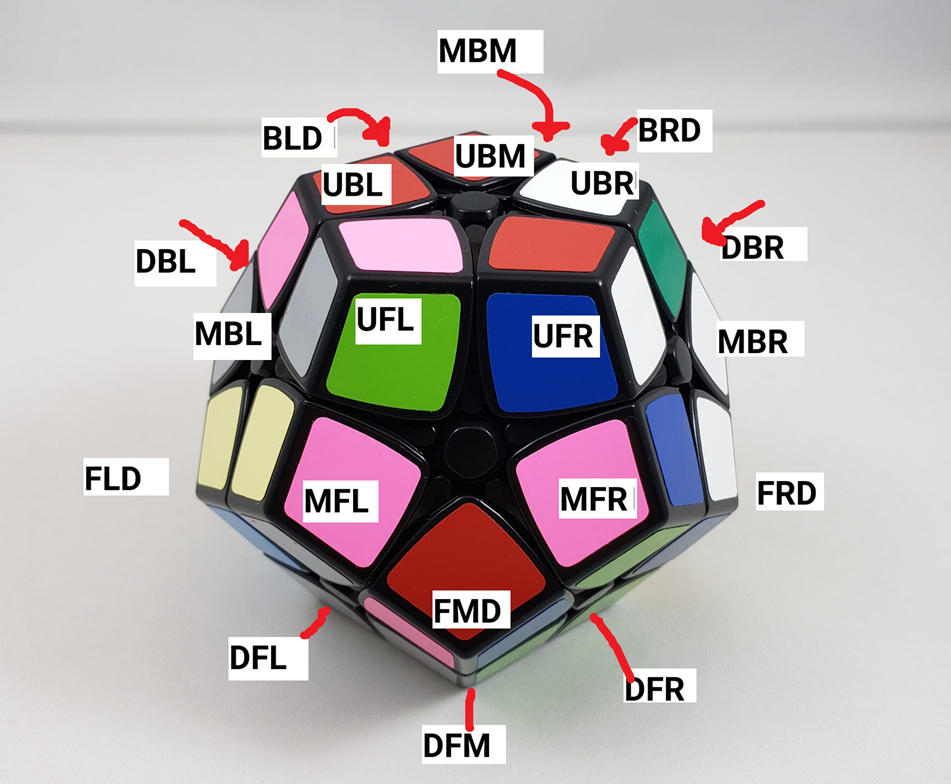
\includegraphics[width=0.8\textwidth]{kilominx_indices_guide}
    \centering
    \caption{An image of a Kilominx, with each cubie labelled based on its position.}
\end{figure}
\label{fig:kubies}

\chapter{User Manual}
% Instructions on installing, executing and using the system
% where appropriate.
\section{Compilation and Running}
The project contains a bash script, `run.sh` which can be used to quickly compile the project, and run any of the available programs based on the provided command-line argument(s). The script must be run from inside the `CS4099` directory (i.e. running the command will look like: '\$ TwistyPuzzleSolvers/run.sh ...'. You might also need to update the execute permissions of the script in order to run it - this can be done using '\$ chmod 777 TwistyPuzzleSolvers/run.sh'. Aside from a recent Java installation, no other dependencies are required. The available arguments are as follows:
\begin{itemize}
    \item 'cube' - Runs the Rubik's Cube terminal program.
    \item 'cube gui' - Runs the Rubik's Cube GUI program.
    \item 'kilominx' - Runs the Kilominx terminal program.
    \item 'pdb [pdb-type]' - Runs the pattern database populator program for the supplied pattern database type.
    \item 'test [scramble-length] [\#-of-test-runs]' - Runs the Kilominx test run program, generating scrambles of the specified length and running the specified number of test runs.
\end{itemize}

\section{Pattern Database Populator}
The pattern database populator takes an argument for the type of pattern database, and then populates that pattern database. Note that for larger pattern databases (such as the Kilominx face pattern databases), the program can take a \textbf{very long time} to finish population (\textbf{over 24 hours}). These pattern databases are \textbf{not} included in the project submission as they are large files (some are roughly 500 MB each), so they need to be manually generated in order for the solvers to work correctly. The available pattern database types are as follows:
\begin{itemize}
    \item 'cube-corners' - For the Rubik's Cube corner cubies pattern database.
    \item 'cube-first-edges' - For the first Rubik's Cube edge cubies pattern database.
    \item 'cube-second-edges' - For the second Rubik's Cube edge cubies pattern database.
    \item 'kilominx-face-\#' (with \# = 1-12) - For a Kilominx face cubies pattern database of the specified set number.
    \item 'kilominx-sparse-\#' (with \# = 1-5) - For the Kilominx sparse cubies pattern database of the specified set number.
\end{itemize}

\section{Rubik's Cube and Kilominx Terminals}
The terminal programs for the Rubik's Cube and Kilominx allow you to make moves and enter commands to interact with the puzzle. The moves for the puzzles are defined above in \textbf{\hyperref[section:moves]{Appendix A}}. The commands are as follows:
\begin{itemize}
    \item HELP - Display a help message.
    \item RESET - Reset the puzzle to the solved state.
    \item EDIT - Enter editing mode.
    \item SCRAMBLE [n] - Scramble the puzzle with n random moves.
    \item SOLVE - Solve the puzzle using the optimal solver.
    \item QUIT - Exit the program.
\end{itemize}
It should be noted that in order to use the SOLVE command, all of the pattern databases associated with the puzzle need to have been generated beforehand - see the previous section for more info on how to do this.

\section{Rubik's Cube GUI}
The GUI program for the Rubik's Cube works in a similar way to the terminal program, but with a coloured display for the cube state and a separate panel to enter terminal commands. The EDIT command is not available in GUI mode.

A number of hotkeys are also defined to quickly make moves on the cube - they can be performed by pressing the face letter on the keyboard. You can also perform counter-clockwise moves by holding down the SHIFT key, and double moves by holding down the CTRL key.

\chapter{Experimental Results}
\label{appendix:results}
The tables below show the full experimental results that were obtained by running the Kilominx solver on pseudo-randomly scrambled states of different scramble lengths, as discussed in \textbf{\hyperref[section:experiment]{Section 7.1}}. The results show the scramble/solution lengths, the lists of moves that make up the scramble/solution, and the solve times. Rows which are highlighted green show test cases where the solver found an optimal solution of a length less than the scramble length. 

\begin{table}[h]
\centering
\resizebox{\textwidth}{!}{%
\begin{tabular}{|p{2cm}|p{7cm}|p{2cm}|p{7cm}|p{2.8cm}|}
\hline
\rowcolor[HTML]{EFEFEF} 
\textbf{Scramble Length} & \textbf{Scramble} & \textbf{Solution Length} & \textbf{Solution} & \textbf{Solve Time (HH:MM:SS)} \\ \hline
10 & DBR2', D2, DL, F, R2, D, DL, D,   DBL', DBR' & 10 & DBR, R2', DBL, D', DL', F',   DBL', DL', D2', DBR2 & 00:00:00 \\ \hline
 & F2, BR2, DB, BR2', R, BR', R2',   BL, U, L2 & 10 & L2', U', R2, BL', BR, R', F2',   D2, DB', D2' & 00:00:01 \\ \hline
 & L2', BL, DBR2', D', DBR, BR, U2,   DBL, DL', DBL' & 10 & U2', DBR, DB, DBR', BR', BL',   L2, DBR', R, DBR2 & 00:00:01 \\ \hline
 & DB2', BR', D', DR2, DB, BL2',   DBL2', DB2', BR', R2' & 10 & R2, BR, DR2', DB2, DBL2, BL2,   DB', BR, D, DB2 & 00:00:00 \\ \hline
 & L2, DL2', DB, D', DBR2', D2',   DBL2, L', DB2, DBL' & 10 & DBL, L, D2', DBL2', D2, DBR2, D,   DL2, L2', R' & 00:00:01 \\ \hline
 & \cellcolor[HTML]{E2EFD9}DR2, R, DB2, DBL, BL, DBL2,   DBR2, BR2', U2, DR2 & \cellcolor[HTML]{E2EFD9}9 & \cellcolor[HTML]{E2EFD9}U2', BR2, DBL, DBR2', R', BL',   DR2', DBL', DB2' & \cellcolor[HTML]{E2EFD9}00:00:00 \\ \hline
 & \cellcolor[HTML]{E2EFD9}U', R2', D, DL', L, BR', DBL2,   DB, D2, DBR2 & \cellcolor[HTML]{E2EFD9}9 & \cellcolor[HTML]{E2EFD9}DBR2', D2', DB', DBL2', L', R2',   U, DR, D' & \cellcolor[HTML]{E2EFD9}00:00:00 \\ \hline
 & \cellcolor[HTML]{E2EFD9}DR2', DBL', L, R, D, DR2', F2',   BL', DBL', BL' & \cellcolor[HTML]{E2EFD9}9 & \cellcolor[HTML]{E2EFD9}F2, L', DB, DBR, DB, D2, DR,   DB', DBL & \cellcolor[HTML]{E2EFD9}00:00:00 \\ \hline
 & DBL2, D2, DBR2', BR, DBL2', BL,   L2', DL', D2', DR2' & 10 & DR2, D2, DL, L2, BL', BR', DBL2,   DBR2, D2', DBL2' & 00:00:00 \\ \hline
 & DR2', R', DBR2', BR, DB, D,   DBR2', DR2', DBL2, BL & 10 & BL', DR2, DBL2', DBR2, D', DB',   BR', DBR2, R, DR2 & 00:00:00 \\ \hline
 &  &  &  &  \\ \hline
11 & BR, R2, F, DBL', L2, D, DB, DBL,   D2', DBL2, DBR2' & 11 & DBL2', DBR2, D2, DBL', L2', R',   F', DBR', R2', BL, BR' & 00:00:05 \\ \hline
 & D, DBR, R2, U2, DBL2', BL2', DR,   DL2, DBR', R2, DBL & 11 & R2', DBL', BL2, U2', DL, DB2',   DBR2, R2', DBL', DBR', D' & 00:00:20 \\ \hline
 & BR', DR2, D2, DL', DR2', DBR',   DR, DBL2, DL2', DR2', DL2 & 11 & DL2', DR2, DL2, DR', DBL2', DBR,   BR, DR2, DL, D2', DR2' & 00:00:26 \\ \hline
 & DR', D2, DL', DBL2', BL2', U2,   DR2, DL2, DR', D2, DBL2' & 11 & U2', DBR2, D2', DBL, DB2',   DBL2', BL2, DBL2, DL, D2', DR & 00:00:34 \\ \hline
 & DBR2', DR2', DL2, DR', D2, DR,   D2', DBR, DR, DBR2, BR & 11 & BR', DBR2', DR', DBR', D2, DR',   D2', DR, DL2', DR2, DBR2 & 00:00:54 \\ \hline
 & BR2, DR, DBL2', DB', DBL, DB,   BL2, DB2', DBL, DB2', BR2' & 11 & BR2, DR', DB2, DBL', DB2, BL2',   DB', DBL', DB, BR2', DBL2 & 00:00:12 \\ \hline
 & BL2', U2', BL2, D, DR, D2',   DBL', D', DBR2', DB2, DBL2 & 11 & DBL2', DB2', DBR2, D, DBL, BL2',   U2, D2, DB', BL2, D' & 00:00:24 \\ \hline
 & DBR2', DB, BL', BR2', DR', D2,   DBL, D, DBL2', D', DB' & 11 & DB, BR2, D, DBL2, D', DBL', BL,   D2', DR, DB', DBR2 & 00:00:26 \\ \hline
 & DR2, DBL, DB2', DBL2', L2', R,   BR', DBR', R', DBL2', BL' & 11 & R, BL, DBL2, L2, DBR, D, DR2',   DB', DBL2, DB2, DBL' & 00:00:12 \\ \hline
 & DB2, DBR', R, F2, BR, DB, D,   DL2', D2', DB, BR' & 11 & BR, DB', D2, DL2, F2', R', BL',   DB', D', DBR, DB2' & 00:00:15 \\ \hline
 &  &  &  &  \\ \hline
12 & U, DBR, D', DL2', L2, F', DBL,   L', DB2', BL', L, DB & 12 & F, DL', DB', D, DL, L2', DBR2,   BR', U', DBL2, D, DR' & 00:01:24 \\ \hline
 & F', BR, BL2', DBL2, BL', DB',   BR2, DB2', D, DR', DL, DB & 12 & DL', DR, F, DB', DBR', DB2,   BL2', DB, DBL, D2', DBL2, BL' & 00:05:08 \\ \hline
 & L2', F2, R, BL2', DR2, DL2,   DB2', D', DBR', D, DB', BL' & 12 & BL, DB, D', DBR, D, DB2, BL2,   DL2', DR2', R', F2', L2 & 00:07:45 \\ \hline
 & L, U', L, U2, L', BR2, BL2,   DR2', DBL, DL', DBL', BL & 12 & BL', DBL, DL, DR2, DBL', BL2',   L, U2', L', U, L', DB2' & 00:06:52 \\ \hline
 & D', DL', L2, DL, DB, DBR2, D,   DBR, DR2, F2', DBL2', DB' & 12 & F2, DB, DBR2, DR2', DBR', D',   DL', L2', DBR2', R', DL, D & 00:01:10 \\ \hline
 & DL, DBR2', BR2, DBR, D, DB',   BL', BR2, DR', R', U', R2 & 12 & R2', U, R, BR2', BL, DR, DB, D',   DBR', BR2', DL', DBR2 & 00:08:59 \\ \hline
 & DR', DBR2', DR2, DB, BL2, U2',   DBR', DR, DB2, DBL', L2', R2' & 12 & L2, U2, DL2, DR, DL2', DR2',   DB', DBL, BL2', DB', DBR2, DR & 00:07:19 \\ \hline
 & DL2, L, BL2, DR2, F', DB2',   BR2', BL2, U', R2', BR, DBL' & 12 & BR', R2, U, BL2', BR2, DB2,   BR2', DL, F, L', D2', DL2' & 00:06:04 \\ \hline
 & F2, L, BL2', DR2, DB2, DBL2',   L', F2', BR2, DBL', DB, D2 & 12 & F2, BR2', DB', DBL2', L, DBL2,   DBR, DB2', BL2, L', F2', BL2' & 00:05:29 \\ \hline
 & BL2, DBR2', DB2, BR, DR2', DL,   DBL2', BL2, DL2', D2', DBR2', BR2 & 12 & BR2', BL2', DBR2, BR', D2, DL2,   DBL2, DB2', BL2', DL', DR2, DBR2 & 00:03:32 \\ \hline
\end{tabular}%
}
\centering
\caption{Kilominx Solver results on pseudo-random scrambled states of lengths 10 to 12.}
\label{tab:results-1}
\end{table}

\begin{table}[h]
\centering
\resizebox{\textwidth}{!}{%
\begin{tabular}{|p{2cm}|p{7cm}|p{2cm}|p{7cm}|p{2.8cm}|}
\hline
\rowcolor[HTML]{EFEFEF} 
\textbf{Scramble Length} & \textbf{Scramble} & \textbf{Solution Length} & \textbf{Solution} & \textbf{Solve Time (HH:MM:SS)} \\ \hline
13 & BR2, BL2, DL2, D', DL2', D, DR',   DBR2', D2, DBR2, BR2', DR2', DB2 & 13 & DR2, DB2', BR2, BL2', DBR2',   D2', DBR2, BR2', DR, D', DL2, D, DL2' & 00:13:54 \\ \hline
 & BL2, U2', R', F', D2', DL, DB',   D2, DBL2, BL', D2', DL, F2 & 13 & F2', BL, DL', D2, DBL2', D2',   DL', F, DB, DBR2, R, U2, BL2' & 01:14:13 \\ \hline
 & \cellcolor[HTML]{C5E0B3}D2, DR2, DBL', DBR', R, DB2,   D2', DBL', DBR, R', U, BR, DL & \cellcolor[HTML]{C5E0B3}11 & \cellcolor[HTML]{C5E0B3}BR', U', R, DBR', R', D2, DB2',   DBR, DR2', DBL, D2' & \cellcolor[HTML]{C5E0B3}00:00:15 \\ \hline
 & U', F, L2', DR2', DB2', DBR2,   BR, DBL2, L2', DL2, DB2, D, DR2' & 13 & DR2, D', DL2', L2, BR', DBL2',   L2, BR2', DBR2', DR2, F', U, DB2 & 02:21:01 \\ \hline
 & DB, BR', U2, R2, BR2, DR, R,   DBR2', BR', DR2', DB, DBL', DB' & 13 & DB, DBL, DB', BR, DR2, DBR2, R',   BR2', DR', R2', U2', BR, DB' & 00:18:52 \\ \hline
 & D, DL2, DBR, BR2', D2', DBL2,   DL2', L, D2', DB2', DBL, DL, L' & 13 & L, DL', DBL', L', BR2, DB2, BR2,   DL2, DBL2', D2, DL2', DBR', D' & 00:50:36 \\ \hline
 & F, R2, DB2', D2', DL2, DB', D2',   DL2, L', DL2', L, F2, DBL & 13 & F2', L', DL2, L, BR', R2', DL2',   D2, DL2', F', DB, DBL2, DB2 & 02:32:11 \\ \hline
 & \cellcolor[HTML]{E2EFD9}BR2, DL', DBR2', BR', BL2', U',   BR, DBL2', DL', D', DR2', D2, DBL2' & \cellcolor[HTML]{E2EFD9}12 & \cellcolor[HTML]{E2EFD9}BR', U, BL2, DL2, D2', DBR2, BR,   D, DR, DBR2, BR2', DL2' & \cellcolor[HTML]{E2EFD9}00:05:56 \\ \hline
 & DBR2', R2, BR2, D', DBR', DB2,   D, DL2', DB2, BL, DR', DB2', D' & 13 & D, DR, DB2, BL', DL2, DB2', D',   DB2', DBR, BR2', R2', D, DBR2 & 00:42:26 \\ \hline
 & DR, F2, BR', BL', U2, BL, DBR2',   BR2', R, F, D', DL, DR' & 13 & DR, DL', F', R', BR2, DBL, BL',   U2', DL2, F2', DBR, D, DR' & 00:47:47 \\ \hline
 & R, DL2', DBL2', DL, DBL2', L2,   U, DR2, DBR, R2, BR', U, R2 & 13 & R2', U', BR, R2', U', DR', DL2',   L2', R', DBL2, DL', DBL2, DL2 & 01:03:20 \\ \hline
 & F2, BL, L2', DBR2, BR2', BL',   D2', DBL, DBR2', DR, DL2, DR2', DB2' & 13 & DR2, DL2', DR', DB2, DBL', BL,   L2, DBR2, R2, F2', BL2, DBL2', DBR' & 02:08:26 \\ \hline
 & D', DBL2, DBR, R2', DB2, DBR',   DB2', D, DR2, DB', D', DL, F' & 13 & F, DL', D, DR2', DB, D', DB2,   DBR, R2, DB2', DBL2', DBR', D & 00:27:15 \\ \hline
 & F', DR2', DL2', F, D, DBR2,   BR2', U, DL2', D2, DR', DL, DBL' & 13 & U', DB, BR2, DBL', DL, F',   DBL2', BL2, D2', DBL', DL2, DR2, F & 01:15:18 \\ \hline
 & \cellcolor[HTML]{E2EFD9}BR, DR, D', DBL', DBR, DR2',   DBL', DB2', BR2', BL2, DB2, BL2, BR & \cellcolor[HTML]{E2EFD9}12 & \cellcolor[HTML]{E2EFD9}BR', BL2', DB2', BL2', BR2, DR2,   DB2, DBR', BR', DBL2, D, DR' & \cellcolor[HTML]{E2EFD9}00:03:50 \\ \hline
 & \cellcolor[HTML]{C5E0B3}BL', BR', D2, DR2, DBL2, L', R,   DB, BR', DBL2, D2', DBR2, DR' & \cellcolor[HTML]{C5E0B3}11 & \cellcolor[HTML]{C5E0B3}DR, DBR2', BR, D2, DBL2', L, D',   DBL2', BL, DR2', D2' & \cellcolor[HTML]{C5E0B3}00:00:03 \\ \hline
 & R2', DL', DR', DL', DB2', DBL2,   DL2, DB', DBR2', DB2', DBR2', DR2, F2' & 13 & F2, DR2', DL', DBR2, DB2, DBR2,   DR, R2, DL', DB, DBL2', DL2, DB2 & 01:46:25 \\ \hline
 & \cellcolor[HTML]{E2EFD9}BR, DBL2', D', DBR2', BR2, DL2,   DR2, DL', F', BL2', DBL2', DBR, BR & \cellcolor[HTML]{E2EFD9}12 & \cellcolor[HTML]{E2EFD9}F, BL', BR2, D2, DBL2, DL, DR2',   DBR2, BR', DL2', D, DBL2 & \cellcolor[HTML]{E2EFD9}00:09:53 \\ \hline
 & DR2, DBL, D', DBL, L2', U2',   BR2, BL2', DR, D2', DBL2, BL2', DB & 13 & DB', BL2, DBL2', BL2, BR2', U2,   L2, R2, DR', DBL', D, DR2', DBL' & 00:53:48 \\ \hline
 & \cellcolor[HTML]{E2EFD9}BL', BR', BL, L, DBL2', L, D2,   DB', DBL2, D, DL2', DBL2, DBR & \cellcolor[HTML]{E2EFD9}12 & \cellcolor[HTML]{E2EFD9}DL, DBR', D2', DBL2', L, DR',   DL2', L2', BL', L', R, BR & \cellcolor[HTML]{E2EFD9}00:05:00 \\ \hline
 & F', DL2, DBL', L', BR', D', DL',   DBL2', DL2, L2, DBL2', L', DL & 13 & DL', L, DBL2, L2', DL2', DBL2,   DL, L, DR, DB, DBL, DL2', F & 01:11:28 \\ \hline
 & BL2, L', DR, D, DBR2, DR2, DL,   DB, BL, DBR2, BR', D2', DL' & 13 & BR, BL', L, F, R2, F', BL2',   DBR2', R2', D', DBR2', DR', R' & 00:22:22 \\ \hline
 & DR', DL2, F2', U2', DR2', DBR,   DB, BR', BL2, BR', U2', R', BR & 13 & BR', R, U2, BR, BL2', BR, U2,   DL', F2, DL2', DBR', DR, DB2 & 01:55:28 \\ \hline
 & U, F', DB, BR, DB, BL2, DR2',   DBL2, DBR', DB2, DBR2', BR2, DR2' & 13 & BR2', DR2, DBR2, DB2', DBR, DR2,   F, D2', DBL2', DB', BL', U', DBR' & 02:36:31 \\ \hline
 & L, DL2, DB, BR2', DR, DB', BL,   D2', DBL2, BL', BR2, DBR', BR2' & 13 & BR2, DBR, BR2', BL, DBL2', BL',   D2, DB, BR2, DR', DL2', L', BR' & 01:55:54 \\ \hline
\end{tabular}%
}
\centering
\caption{Kilominx Solver results on pseudo-random scrambled states of length 13 (first half).}
\label{tab:results-2}
\end{table}

\begin{table}[h]
\centering
\resizebox{\textwidth}{!}{%
\begin{tabular}{|p{2cm}|p{7cm}|p{2cm}|p{7cm}|p{2.8cm}|}
\hline
\rowcolor[HTML]{EFEFEF} 
\textbf{Scramble Length} & \textbf{Scramble} & \textbf{Solution Length} & \textbf{Solution} & \textbf{Solve Time (HH:MM:SS)} \\ \hline
 13 & DBR2, R, D2', DBR', R2', BL',   DBL, D, DB2', BL2, DBR, DR2', R2 & 13 & R2', BL2', DR2, DBR', R2, DB2,   D', DBR, R', DBL', BL, D2, DBR2' & 03:52:22 \\ \hline
 & DBR2', D2', DBR, DB, DBL', DB',   D', DB', BR2', DR2, R2', U2, F2 & 13 & F2', U2', R2, BR2, DR2', DB, D,   DB, DBL, DB', DBR', D2, DBR2 & 00:47:58 \\ \hline
 & U', DBR, BR2, D', DBR2, DB, BL,   D2, DL, DBL', DL, DB, D' & 13 & D, DL', DB', DBL, BL', DL', D2',   DB', DBR2', BR2', U, D, DB' & 04:14:35 \\ \hline
 & DBL2', DBR2, D, DR2', DBL, DB,   DBL2, DB2, BR2, DB2, D', DB', DBR & 13 & DBR', DB, D, DR2, DB2', BR2',   DB2', DBL2', DB', DBL', D', DBL2, DBR2' & 03:44:57 \\ \hline
 & DBR', DR', DBL2', L2, U2, BL,   DBR, D2', DBR2, DR', D, DBR2', DB' & 13 & DB, BL', U2', BR, DL2, D', DBL,   DL2', D2, DL', L2', DBL2, DBR & 02:38:15 \\ \hline
 & DBR2, R, DL2', F2, DBL', DB,   DBL, L, BR2', D', DB', BL2, DL2' & 13 & BL2', DB, BR2, DL2, L', F2',   DL2, DB, BR', DB', BR, R', DBR2' & 00:22:15 \\ \hline
 & DBL', D', DR2, DB, DBR, DB2',   DBL2, DL2', DBL2, L, R2', DBR, DR & 13 & L', D', DBR', DR2, DBL2', DL2,   DBL2', DB2, DBR', DR2', DB', D, DBL & 03:40:56 \\ \hline
 & DBR2', DB2', DBR, R2', DR, D',   DR, D', DB', D2, DR2, DBR2', D2 & 13 & D2', DBR2, DR2', D2', DB, D,   DR', D, DR', R2, DBR', DB2, DBR2 & 03:48:56 \\ \hline
 & DL2, D2, DR2, DBL, L2, DR2, R',   DBR2', DR, DBL2, D2, DBL2', BL2' & 13 & BL2, DBL2, D2', DR', DBR2, R,   BR2', DBL2', L2', DB2', DBL', D2', DL2' & 02:12:32 \\ \hline
 & D, DL2', DR', D', DL2', DB2,   BR', DB2, DBL2, DB2, BL2, DL2, L & 13 & L', BL2', DL2', DB2', DBL2',   DB2', BR, DL2, DB2', D, DR, DL2, D' & 01:41:29 \\ \hline
 & \cellcolor[HTML]{C5E0B3}DR2, DB', BL, DR2', F, R2, DB',   BL2', DBR', R2', DR2, DBL', DB2' & \cellcolor[HTML]{C5E0B3}11 & \cellcolor[HTML]{C5E0B3}DR2', R2, DB2, DBR, R2', F', BL,   BR2, DB, BL', DB & \cellcolor[HTML]{C5E0B3}00:00:24 \\ \hline
 & DBL2, D2, DL, DB2', BL, DBL2,   DB', DBL2, DL', DBL2, DB2, BR', DR' & 13 & BR, DBR', DB2', DBL, DB2', DBR,   DB2', DBL2', BL', DR, DB2, D2', DBL2' & 04:22:24 \\ \hline
 & \cellcolor[HTML]{E2EFD9}BL2, DB, BR, DR, DBL', L2',   DBL', L', BR, U2', BL', D2, DBL2' & \cellcolor[HTML]{E2EFD9}12 & \cellcolor[HTML]{E2EFD9}DBL2, BL, U2, L, DR2, DB', DBL,   L2, DBL, DB', BL2', DR' & \cellcolor[HTML]{E2EFD9}00:07:21 \\ \hline
 & R2, DR', F2, DBR2', DR, DBL,   D2', DR, DL', D2, DL2, DR2, DBL2' & 13 & DR2', DBL2, DL2', D2', DL, DR',   D2, DR', F2', BR', DR, R2', DBL2 & 00:36:13 \\ \hline
 & L, DBR, DR', D2, DBL, BL2', DL,   DR2', D, DBL', D, DL', DBR2 & 13 & DL, DBR2', D', DBL, BL2, D',   DR2, DL', DBL', L', DB2', D, DBR' & 02:11:12 \\ \hline
 & U, DB, BR', DBL2', BL', D2, DB',   BL2, BR', U, DL, F, DB2' & 13 & F', U', DBL', DBR2, BR, BL2',   DB, BL, BR, U', D2', DB2, DBR' & 01:53:43 \\ \hline
 & DBR', D', DR', F', R2', DBL2',   L2', R2, DBR2, DB', DBR2', R2', DBL2 & 13 & R2, DBL2', L2, DBR2, DR, DBR2',   R2, F, DB2', D2, DR, D, DBR & 02:07:46 \\ \hline
 & DL2', F2', U, R2', DBL2', DB',   BL2, L2', F2, DB2', D2, DBR', DR & 13 & DR', F2', DBL, BL2', L2, DR2,   R2, BL2', U', F2, BL, DL2, DB2 & 03:12:47 \\ \hline
 & D, DB2', BL2, D2, DL', DBL2',   D2, DB', DBL', DB', D', DR', F' & 13 & F, DR, D, DB, DBL, DB, D2',   DBL2, BL2', DL, D2', DB2, D' & 03:56:32 \\ \hline
 & \cellcolor[HTML]{C5E0B3}U2, L', BL2, U, R2', DL2, L2,   R', F, DB2, D2', DBL2', DB2' & \cellcolor[HTML]{C5E0B3}11 & \cellcolor[HTML]{C5E0B3}F', DB2, BL2, DBL2, L2', U', D,   DBL2', BL2', L, U2' & \cellcolor[HTML]{C5E0B3}00:00:18 \\ \hline
 & DL2, DR2, DBR', BR2, DR2, DBR',   D, DL2', DR', F, BL', DBL2, DL2 & 13 & DL2', F', BL2', BR, DR, DL2, D',   DBR, BR2', DR2', DBR, DR2', DL2' & 00:25:09 \\ \hline
 & DB2, BL', DR2', D2, DL2, DBR',   DR2', DBL2', BL, L, DB, DBL2', L2 & 13 & L2', R2, DBL2, L', BR', BL',   DBL2, BL, DL2', DBR, D2', DR2, DB2' & 04:41:21 \\ \hline
 & DR2', DBR, DR', F, DL, DBL', L,   DL2, D', DBR', R, U', DL2' & 13 & U, DR2, R', DBR, D, DL2', L',   DBL, DL', F', DR, DBR', DR2 & 04:59:39 \\ \hline
 & \cellcolor[HTML]{E2EFD9}DR', R2', DR2, DBR2, D', DL',   DBR2, DB', BR2, DL', L', F', DL2' & \cellcolor[HTML]{E2EFD9}12 & \cellcolor[HTML]{E2EFD9}DL2, F, L, BR2', DL2, DB, DBR2',   D, DBR2', DR2', R2, DR & \cellcolor[HTML]{E2EFD9}00:03:32 \\ \hline
 & DB2', DBR2, R2, D', DB, DBL2,   DL, DBL2, DL', D, DBR', D, DBL2 & 13 & DBL2', D', DBR, R2', D', DL,   DBL2', DL', DBL2', DB', D, DBR2', DB2 & 04:25:09 \\ \hline
\end{tabular}%
}
\centering
\caption{Kilominx Solver results on pseudo-random scrambled states of length 13 (second half).}
\label{tab:results-3}
\end{table}

\begin{table}[h]
\centering
\resizebox{\textwidth}{!}{%
\begin{tabular}{|p{2cm}|p{7cm}|p{2cm}|p{7cm}|p{2.8cm}|}
\hline
\rowcolor[HTML]{EFEFEF} 
\textbf{Scramble Length} & \textbf{Scramble} & \textbf{Solution Length} & \textbf{Solution} & \textbf{Solve Time (HH:MM:SS)} \\ \hline
14 & BR, BL2', BR', R2, DR2, D',   DB2', DBR', DB2, DBR2, BR', DR, DBR', DR' & 14 & DR, DBR, BR, DR', DBR2', DB2',   DBR, DB2, D, DR2', R2', BR, BL2, BR' & 52:46:10 \\ \hline
 & DB', BL2, DR', DBR2, DB2', DBL',   BL2', L, F2', U', DR', DL, DBL', L2' & 14 & L2, U, DL, DR', F2, BL, L', BL2,   DBL, DB2, BL2', DBR2', DR, DB & 14:11:03 \\ \hline
\end{tabular}%
}
\centering
\caption{Kilominx Solver results on pseudo-random scrambled states of length 14.}
\label{tab:results-4}
\end{table}

\chapter{Artefact Evaluation Form}
\label{appendix:artefact}
\begin{figure}[h]
    
\includegraphics[width=0.8\textwidth]{Ethics.pdf}
    \centering
    \caption{The artefact evaluation form.}
\end{figure}

\printbibliography[heading=bibintoc, title={References}]

\end{document}
